\documentclass[11pt]{scrartcl}
\usepackage[T1]{fontenc}
\usepackage[utf8]{inputenc}

\title{Computer Systems Week 4 Lab}
\author{Daniel Coady (102084174)}
\date{01/09/2019}

\usepackage{graphicx}

\begin{document}

\maketitle

\section*{Theory Questions}

\subsection*{What is ROM and what is its primary purpose?}
ROM is short for "Read Only Memory" and as the name implies, it is memory that you
can only read from. ROM is generally used for things like storing the BIOS of a 
system since you only want to be reading from it where writing over it could be
potentially catastrophic to the system's operation.

\subsection*{What is RAM and how is it different from ROM?}
RAM is short for "Random Access Memory", which as the name insists allows for
quick random access of information from memory. The main difference between it
and ROM is that RAM is volatile, meaning that it loses all information when it
loses power, which ROM is non-volatile.

\subsection*{What is the difference between static RAM and dynamic RAM?}
The main differences between the two types of RAM are that static RAM loses its
state once it loses power while dynamic RAM keeps its state as long as it is
periodically given more power and static RAM requires a larger area of silicon
per byte compared to dynamic RAM.

\subsection*{What type of memory is typically used in USB thumb drives? Why
             shouldn't we rely on this for critical data storage?}
USB drives typically use a type of memory called electrical erasable read only
memory, or EEPROM for short. Over time, the memory itself will degrade and then
eventually fail. This can be mitigated somewhat by use of wear levelling logic
but eventually it will finally fail, losing access to any data you may have had on
the drive which makes it not very suitable for critical data storage.

\subsection*{Consider a computer with 1GB of RAM (1024MB). Given memory addressing
             is for each byte, how many bits are needed to address all bytes in the
             system's RAM?}
You would require 30 bits to address every word in the 1GB of RAM. This can be
calculated with the formula log2(n), where is the amount of bytes being addressed.

\subsection*{Give a brief description of the Von Neumann and Harvard computing
             architectures. What are the fundamental differences between the two
             and for what is each designed to achieve?}
The high level difference between the two architectures is that Von Nuemann stores the
instruction memory and data memory in the same location while the Harvard architecture
stores it in two separate physical areas of memory. Von Nuemann allows for cheaper and
more extensible production but has both speed and security issues because of the shared
memory space and bus. Harvard then solves this with the two separate physical areas of
memory which also inherently means that there are two separate buses for the two areas
of memory. This offers both security and speed but then sacrifices the extensibility of
the architecture, which in turn makes it more expensive to produce.

\subsection*{What is cache memory and what is its primary role?}
Cache memory is memory that is stored extremely close to the CPU, giving it easy and
fast access to it. Cache memory is generally used for anything that the CPU needs quick
access to such as recently used variables.

\subsection*{Explain the concept of an interrupt and list four common types}
Interrupts are how we can better interact with hardware such as peripherals that might
be connected to your system. It works by the device sending an interrupt signal to the
CPU which will then stop what it's doing to handle the interrupt. Common types of
interrupts include:
\begin{itemize}
    \item Errors
    \item Input devices (mouse/keyboard)
    \item Networking
    \item Exceptions
\end{itemize}

\subsection*{Briefly explain polling and why it is not commonly used}
Polling is an alternative to how interrupts work. Instead of handling interrupts as
they come in, polling works by essentially "checking in" with each component to see
how things are going at a fixed rate. If anything needs to have something handled, then
the CPU will handle it. Because polling happens at a constant rate, this means that it is
always using CPU time as opposed to interrupts which will only use CPU time as it is
required.

\subsection*{Explain the general concept of a stack -- how do they work, and what is
             their primary purpose}
Stacks are a data structure that allows you to store a collection of data. It works by
pushing data on top of the stack and then popping it off the top. Stacks are very common
when we want to store a set of instructions that we wish to execute in a specific order.

\subsection*{How are stacks useful for handling interrupts?}
When an interrupt signal is recieved the CPU will actually push the current task it is working
on to the stack so it can access it later. When it is done handling the interrupt it will then
pop the next task off the stack so it can continue where it left off before.

\subsection*{How are stacks useful in programming?}
Stacks in programming are useful if you have a particular way you wish to be able to access the
data within a collection, like for example if you wanted to program in a deck of cards that you
are able to draw only from the top of.

\section*{Practical Questions}

\begin{figure}[h]
    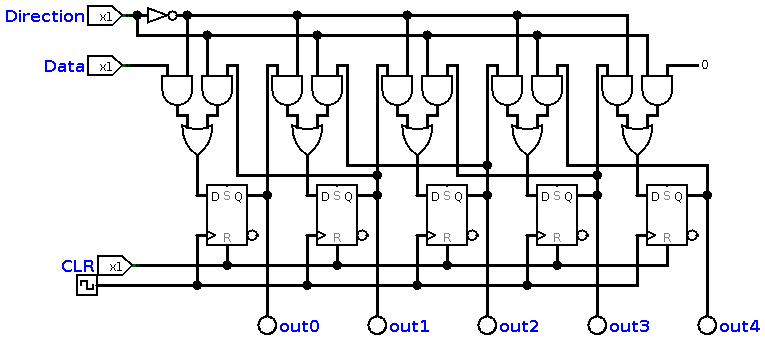
\includegraphics[scale=0.5]{images/stack.png}
    \caption{5 bit deep 1 bit wide stack}
\end{figure}

\pagebreak

\begin{figure}[h]
    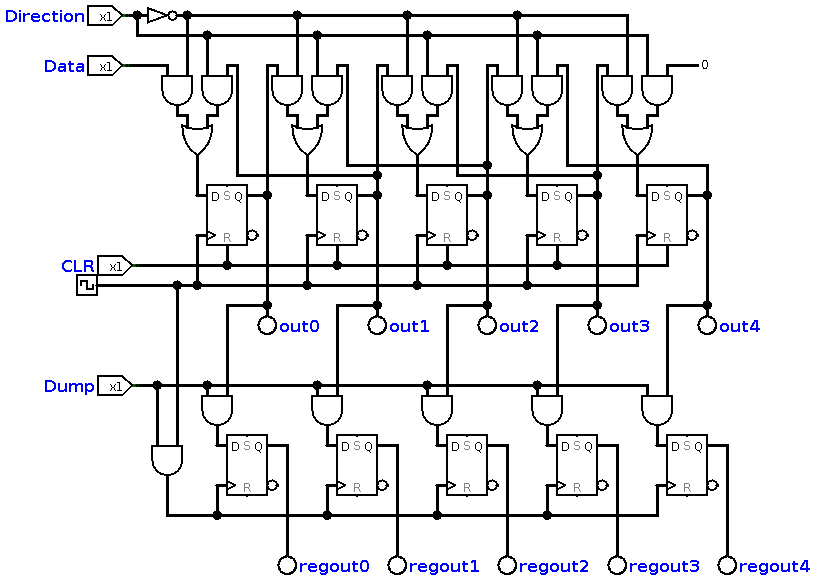
\includegraphics[scale=0.5]{images/stackdump.png}
    \caption{5 bit deep 1 bit wide stack with parallel dump to register}
\end{figure}

\end{document}
